% Created 2016-07-06 Wed 10:08
\documentclass[12pt,t,xcolor=table]{beamer}

\input{/home/stephan/H/Styles/style_presentation.tex}
\usetheme{default}
\author{Stephan Lindner}
\date{6/7/2016}
\title{Exacloud: An Overview}
\begin{document}

\maketitle

\section{Introduction / Overview}
\label{sec:orgheadline3}

\begin{frame}[label={sec:orgheadline1}]{Goals of this presentation}
\vspace{1em}

\begin{itemize}
\item Give an overview of Exacloud and how we can use it.\setlength\itemsep{0.5em}

\item Provide a foundation for discussion regarding how to move forward with Exacloud server.

\item Stay away from more complicated, technical aspects.
\end{itemize}
\end{frame}

\begin{frame}[label={sec:orgheadline2}]{Outline}
\vspace{1em}

\begin{enumerate}
\item What is Exacloud?\setlength\itemsep{0.5em}

\item Accessing and navigating Exacloud.

\item Interactive and non-interactice use of Exacloud.
\end{enumerate}
\end{frame}

\section{What is Exacloud? And why is it on a Linux server?}
\label{sec:orgheadline8}
\setcounter{section}{1}
\begin{frame}[c]{}
  \begin{itemize}
    \item[\bf\thesection.] \bf\insertsection
  \end{itemize}          
\end{frame}

\begin{frame}[label={sec:orgheadline4}]{What is Exacloud?}
\vspace{1em}

\begin{itemize}
\item Exacloud a server run by OHSU's Advanced Computing Center to support large-scale, computational and data intense workflows.\setlength\itemsep{0.5em}

\item Currently more than 35 Terabytes of memory and more than 750 Terabytes of usable storage.

\item Housed at the Data Center at OHSU's West Campus.\vspace{0.5em}
\end{itemize}

\vspace{1em}
\begin{center}
  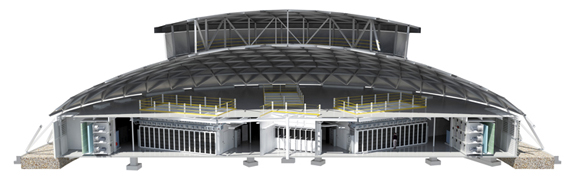
\includegraphics[width=.8\textwidth]{Figures/ohsu-datacenter.png}
\end{center}
\end{frame}


\begin{frame}[label={sec:orgheadline5}]{Exacloud and Linux}
\vspace{0.5em}

\begin{itemize}
\item Exacloud uses Linux as operating system.\setlength\itemsep{0.5em}

\item By contrast, the CHSE server (and our computers) use Windows as operating system.

\item An operating system is the software that manages a computer's basic functioning --- the ``habitat of your programs''.

\item Linux and Windows get along OK, but they do not particularly like each other.

\item Most programs (such as R, Stata) are developed for both operating systems.
\end{itemize}
\end{frame}

\begin{frame}[label={sec:orgheadline6}]{Why does Exacloud uses Linux?}
\vspace{0.5em}

Linux is \ldots{}

\begin{itemize}
\item Very stable.\setlength\itemsep{0.5em}

\item Slim and scalable and therefore has less hardware requirements.

\item Designed as a multi-user system.

\item More secure than Windows.

\item FOSS (Free and Open Source Software).
\end{itemize}
\end{frame}

\begin{frame}[fragile,label={sec:orgheadline7}]{What this mean for us}
 \vspace{1.0em}

\begin{itemize}
\item Many programs we use for our analysis are open-source, have been developed on Linux and work very well on Exacloud: \texttt{R}, \texttt{git}, \texttt{markdown}.\setlength\itemsep{0.5em}

\item \texttt{RStudio} and \texttt{Stata} are not open-source and native to Linux. They are currently not installed on Exacloud.

\item Accessing Exacloud is different from accessing the CHSE server.
\end{itemize}
\end{frame}

\section{Accessing and navigating Exacloud}
\label{sec:orgheadline12}
\begin{frame}[c]{}
  \begin{itemize}
    \item[\bf\thesection.] \bf\insertsection
  \end{itemize}          
\end{frame}

\begin{frame}[fragile,label={sec:orgheadline9}]{Accessing Exacloud via ssh}
 \vspace{1.0em}

\begin{itemize}
\item Remote access of CHSE server: through Windows desktop.\setlength\itemsep{0.5em}

\item Remote access of Exacloud: through \texttt{ssh} (secure shell).

\item \texttt{Shell} is a command prompt to interact with the computer (e.g., start or terminate programs).

\item Bare-bone, 1970 technology that requires very little memory.
\end{itemize}
\end{frame}

\begin{frame}[fragile,label={sec:orgheadline10}]{MobaXterm: ssh for Windows}
 \vspace{1.0em}

\begin{itemize}
\item Install \texttt{MobaXterm} on desktop.\setlength\itemsep{0.5em}

\item Initiate ssh session with 
\begin{itemize}
\item Remote host: \texttt{exacloud.ohsu.edu}
\item User name: \texttt{your OHSU user name}.
\end{itemize}

\item Prompts for password and then connects to server.
\end{itemize}
\end{frame}

\begin{frame}[fragile,label={sec:orgheadline11}]{Navigating Exacloud}
 \vspace{0.5em}

A couple of useful commands:\setlength\itemsep{0.5em}

\begin{itemize}
\item Printing the working directory: \texttt{pwd}

\item Listing files in current directory: \texttt{ls (-lh / -a)}

\item Start \texttt{R}: \texttt{R}

\item Start \texttt{Stata}: \texttt{stata} (currently not installed).

\item Work with \texttt{HTcondor}: \texttt{condor\_submit}, \texttt{condor\_q}
\end{itemize}


\vspace{1em}

\emph{Switch to MobaXterm}
\end{frame}

\section{Interactive and non-interactive use of Exacloud}
\label{sec:orgheadline23}
\begin{frame}[c]{}
  \begin{itemize}
    \item[\bf\thesection.] \bf\insertsection
  \end{itemize}          
\end{frame}

\begin{frame}[fragile,label={sec:orgheadline13}]{Interactive versus non-interactive R / Stata session:}
 \begin{block}{1. Interactive:}
\begin{itemize}
\item Workflow: Develop some code chunk in script file \(\rightarrow\) evaluate code in \texttt{R} / \texttt{Stata} \(\rightarrow\) revise / debug code \(\rightarrow\) \ldots{} \setlength\itemsep{0.5em}\vspace{-1.0em}

\item Setup: Umbrella program that integrates editor with statistical program: \texttt{RStudio}, \texttt{Stata}'s GUI, etc.

\item Requirement: Umbrella program needs to be able to send code chunks to \texttt{R} / \texttt{Stata} and display results.
\end{itemize}
\end{block}
\end{frame}

\begin{frame}[fragile,label={sec:orgheadline14}]{Interactive versus non-interactive R / Stata session:}
 \begin{block}{2. Non-interactive mode:}
\begin{itemize}
\item Workflow: Write full script file \(\rightarrow\) run full script in \texttt{R} / \texttt{Stata} \(\rightarrow\) revise / debug \(\rightarrow\) \ldots{} \setlength\itemsep{0.5em}

\item Setup: Call script file through umbrella program / shell (in \texttt{R}: \texttt{Rscript}).

\item Requirements: some way to call \texttt{R} / \texttt{Stata} from command line.
\end{itemize}
\end{block}
\end{frame}

\begin{frame}[label={sec:orgheadline15}]{Interactive mode on servers:}
\begin{block}{Option 1:}
\emph{Run umbrella program and R / Stata on server.}

\begin{itemize}
\item This is how we use the CHSE server.\setlength\itemsep{0.5em}

\item Requires a lot of data traffic between remote server and local computer.

\item Not possible for Exacloud server because it does not have a desktop environment.
\end{itemize}
\end{block}
\end{frame}

\begin{frame}[label={sec:orgheadline16}]{Interactive mode on servers:}
\begin{block}{Option 2:}
\emph{Run umbrella program locally, R / Stata on server.}

\begin{itemize}
\item Requires little data traffic between remote server and local computer.\setlength\itemsep{0.5em}

\item Umbrella program needs to be able to transfer code / results back and forth between local computer and server.

\item Possible for Exacloud, depending on umbrella program:

\begin{itemize}
\item Rstudio: No

\item Stata: ?

\item Emacs: Yes :)
\end{itemize}
\end{itemize}
\end{block}
\end{frame}

\begin{frame}[fragile,label={sec:orgheadline17}]{Non-interactive mode: a simple example}
 \vspace{1em}

\begin{enumerate}
\item Write \texttt{.R} file (\emph{example1.R}): \setlength\itemsep{0.5em}

\begin{minted}[fontsize=\footnotesize,baselinestretch=1,bgcolor=mintedbg]{r}
x <- 1:1000
summary(x)
\end{minted}

\item Evaluate \texttt{.R} file using \texttt{Rscript}: 

\begin{minted}[fontsize=\footnotesize,baselinestretch=1,bgcolor=mintedbg]{shell}
Rscript example1.R
\end{minted}
\end{enumerate}
\end{frame}

\begin{frame}[fragile,label={sec:orgheadline18}]{Non-interactive mode: processing R markdown file}
 \vspace{0.5em}

\begin{itemize}
\item An \texttt{.Rmd} file has text and source code.\setlength\itemsep{0.5em}

\item \texttt{knitR} evaluates the \texttt{R} source blocks and creates \texttt{markdown} file.

\item In interactive mode, simply call \texttt{knit(file.Rmd)} in \texttt{R}.

\item Does not work in non-interactive mode because \texttt{Rscript} does not accept \texttt{.Rmd} as input file.

\item Solution: write \texttt{R} script file that calls \texttt{knit} to evaluate \texttt{.Rmd} file.
\end{itemize}
\end{frame}

\begin{frame}[fragile,label={sec:orgheadline19}]{Non-interactive mode: processing R markdown file}
 \begin{enumerate}
\item Write \texttt{.Rmd} file (\emph{example1.Rmd}): \setlength\itemsep{0.5em}

\begin{minted}[fontsize=\footnotesize,baselinestretch=1,bgcolor=mintedbg]{rd}
Example markdown file

```{r}
 x <- 1:1000
 summary(x)
```
\end{minted}

\item Write \texttt{.R} file that evaluates \texttt{.Rmd} file (\emph{master-knitr.R}):

\begin{minted}[fontsize=\footnotesize,baselinestretch=1,bgcolor=mintedbg]{r}
library(knitr)
library(rmarkdown)
knit(commandArgs(TRUE)[1])
\end{minted}

\item Evaluate \texttt{.R} file using \texttt{Rscript}: 

\begin{minted}[fontsize=\footnotesize,baselinestretch=1,bgcolor=mintedbg]{shell}
Rscript master-knitr.R example1.Rmd
\end{minted}
\end{enumerate}
\end{frame}

\begin{frame}[fragile,label={sec:orgheadline20}]{Non-interactive mode on Exacloud: HTCondor}
 \vspace{0.5em}

\begin{itemize}
\item Purpose: Efficiently allocate resources to processes that run on decentralized computing system such as Exacloud.\setlength\itemsep{0.75em}

\item Basic usage is pretty simple: 

\begin{enumerate}
\item Write a submit file that tells \texttt{HTCondor} which program to run.

\item Submit the request to \texttt{HTCondor}.
\end{enumerate}

\item There is a lot we could do with \texttt{HTCondor}:

\begin{itemize}
\item Request memory for job.

\item Run script files in different directories.

\item Use macros, conditionals, \ldots{}
\end{itemize}
\end{itemize}
\end{frame}

\begin{frame}[fragile,label={sec:orgheadline21}]{Non-interactive mode using HTCondor}
 \vspace{0.5em}

\begin{enumerate}
\item Write \texttt{.Rmd} file (\emph{example1.Rmd}): \setlength\itemsep{0.3em}

\begin{minted}[fontsize=\footnotesize,baselinestretch=1,bgcolor=mintedbg]{rd}
Example markdown file

```{r}
 x <- 1:1000
 summary(x)
```
\end{minted}

\item Write \texttt{.R} file to evaluate \texttt{.Rmd} file (\emph{example1.R}): 

\begin{minted}[fontsize=\footnotesize,baselinestretch=1,bgcolor=mintedbg]{r}
library(knitr); library(rmarkdown)
knit(commandArgs(TRUE)[1])
\end{minted}

\item Write \texttt{HTCondor} file to evaluate \texttt{.R} file (\emph{examples.htc}):

\begin{minted}[fontsize=\footnotesize,baselinestretch=1,bgcolor=mintedbg]{text}
Executable        = /usr/bin/Rscript
Arguments         = "master-knitr.R example1.Rmd"
\end{minted}

\item Run file:

\begin{minted}[fontsize=\footnotesize,baselinestretch=1,bgcolor=mintedbg]{shell}
condor_submit examples.htc
\end{minted}
\end{enumerate}
\end{frame}

\begin{frame}[fragile,label={sec:orgheadline22}]{Complete sequence to evaluate .Rmd script on Exacloud:}
 \vspace{1.0em}

\begin{enumerate}
\item Submit file to \texttt{HTCondor}.\setlength\itemsep{0.5em}

\item \texttt{HTCondor} calls \texttt{Rscript}.

\item \texttt{Rscript} evaluates \texttt{master-knitr.R}.

\item \texttt{master-knitr.R} calls \texttt{knit} to evaluate \texttt{.Rmd} file.

\item Resulting markdown file can be downloaded and exported to html / pdf.
\end{enumerate}
\end{frame}
\end{document}